\documentclass[11pt]{beamer}
%\documentclass[a4paper,presentation]{beamer}
\usefonttheme{professionalfonts}
\usefonttheme{serif}

\usepackage{eurosym}
\usepackage{ifthen}
\usepackage[utf8]{inputenc}
\usepackage[french]{babel}
\usepackage[T1]{fontenc}
\usepackage{graphicx}
\usepackage{framed}
\usepackage{moreverb}
\usepackage{multicol}
\usepackage[linesnumbered,ruled,vlined,onelanguage]{algorithm2e}
\usepackage{latexsym}
\usepackage{exscale}
\usepackage{graphicx} 
\usepackage{amssymb}
\usepackage{amsmath}
\usepackage{ragged2e}
\usepackage{amsbsy}
%\usepackage{pgfpages}
%\mode<handout>{\setbeamercolor{background canvas}{bg=black!20}}
%\pgfpagesuselayout{2 on 1}[letterpaper,border shrink=5mm]

%\usepackage{amsopn}
%\DeclareMathOperator{\supp}{supp}

%\usepackage{pdfpages}

%\usetheme{CambridgeUS} % 2.5d red/grey
%\usetheme{PaloAlto}
%\usetheme{Frankfurt} % 3d blue/black
%\usetheme{Luebeck} % 2d blue/black
%\usetheme{Madrid} % 2.5d blue
%\usetheme{Rochester} % 2d blue
%\usetheme{Singapore} % blue shade at top, plain
%\usetheme{Warsaw} % 3d blue/black
\usetheme{Darmstadt}
\usecolortheme{rose}
%%%%%%%%%%%%%%%%%%%%%%%%
\definecolor{mine}{RGB}{247,251,249}
\setbeamercolor{background canvas}{bg=mine!50!mine}

%%%%%%%%%%%%%%%

% \AtBeginSubsection[]
% {
%   \begin{frame}<beamer>
%     \frametitle{Structure}
%     \tableofcontents[currentsection,currentsubsection]
%   \end{frame}
% }

\AtBeginSection[]
{
  \begin{frame}<beamer>
    \frametitle{Plan}
    \tableofcontents[currentsection]
  \end{frame}
}

%\title[Data Warehouse]{Entrepôt de Données  \\ Conception et Implémentation }
%\author{Ziyati Houssaine}
%\institute[UH2C]{Université Hassan II  \\ Fsak, Casa}
%\date{\today}

\title[Machine Learning]{Machine Learning \\ Introduction à l’Apprentissage Supervisé }
\small \author{Y. Chafiqui}

\huge
\institute[ESTC]{}
\date{\today}

\begin{document}
%%%%%%%%%%%%%%%%%%% Beginning %%%%%%%%%%%%%%%%%%%
\begin{frame}
  \titlepage
\end{frame}

\begin{frame}
  \frametitle{Plan}
  \tableofcontents

\end{frame}

\section{Introduction à l’Apprentissage Supervisé}

\subsection[Définition de l’apprentissage supervisé]{Définition de l’apprentissage supervisé}

\begin{frame}
  \frametitle{Introduction à l’Apprentissage Supervisé}
 
  \setbeamercolor{block title}{use=structure,fg=white,bg=blue!75!black}
  \setbeamercolor{block body}{use=structure,fg=black,bg=white!20!white}
 
  \large
\uncover<1->{  
  \begin{block}{Qu’est-ce que l’apprentissage supervisé ?}
L'apprentissage supervisé est un type d’apprentissage automatique (Machine Learning) où on entraîne un modèle avec des données étiquetées et le modèle apprend à prédire des résultats.


\end{block}
}
\pause
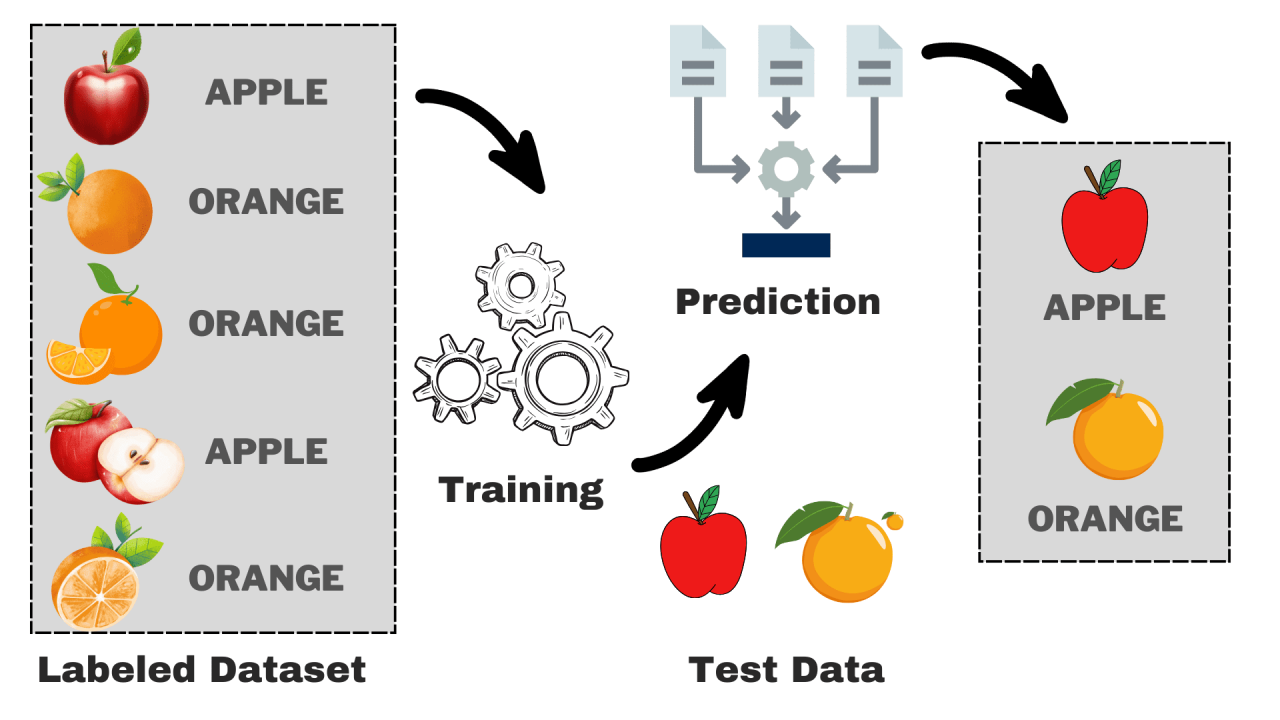
\includegraphics[scale=0.2]{images/supervised ml.png} 
\end{frame}

\begin{frame}
%\setbeamercolor{block title}{use=structure,fg=white,bg=green!75!black}
%\setbeamercolor{block body}{use=structure,fg=black,bg=white!20!white}
  \frametitle{}
  \uncover<1->{
    \begin{block}{Concepts Clés} 
    	\begin{itemize}
    	\item Caractéristiques (features) : Variables d’entrée (ex : âge, salaire)
    	\item Étiquettes (labels) : Résultat attendu (ex : achat = oui/non)
    	\item Entraînement : Le modèle apprend
    	\item Test : On vérifie les résultats sur de nouvelles données
    	\end{itemize}
    \end{block}
  }
\end{frame}

\subsection[Types d’Apprentissage Supervisé]{Types d’Apprentissage Supervisé}
\begin{frame}
%\setbeamercolor{block title}{use=structure,fg=white,bg=blue!75!black}
%\setbeamercolor{block body}{use=structure,fg=black,bg=white!20!white}
  \frametitle{Types d’Apprentissage Supervisé}
  \uncover<2->{
    \begin{block}{Classification} 
    \begin{itemize}
    \item Le modèle est entraîné pour prédire une catégorie de valeurs...
    \item Ex : Email spam ou non spam	
    \end{itemize}
    \end{block}
  }
%\setbeamercolor{block title}{use=structure,fg=white,bg=magenta!75!black}
%\setbeamercolor{block body}{use=structure,fg=black,bg=white!20!white}
  \uncover<3->{
    \begin{block}
      {Régression}
      \begin{itemize}
        \item Le modèle est entraîné pour prédire une valeur continue...
        \item Ex : Prix d’une maison
      \end{itemize}
    \end{block}
  }
\end{frame}

\begin{frame}
\frametitle{Types d’Apprentissage Supervisé}
\begin{center}
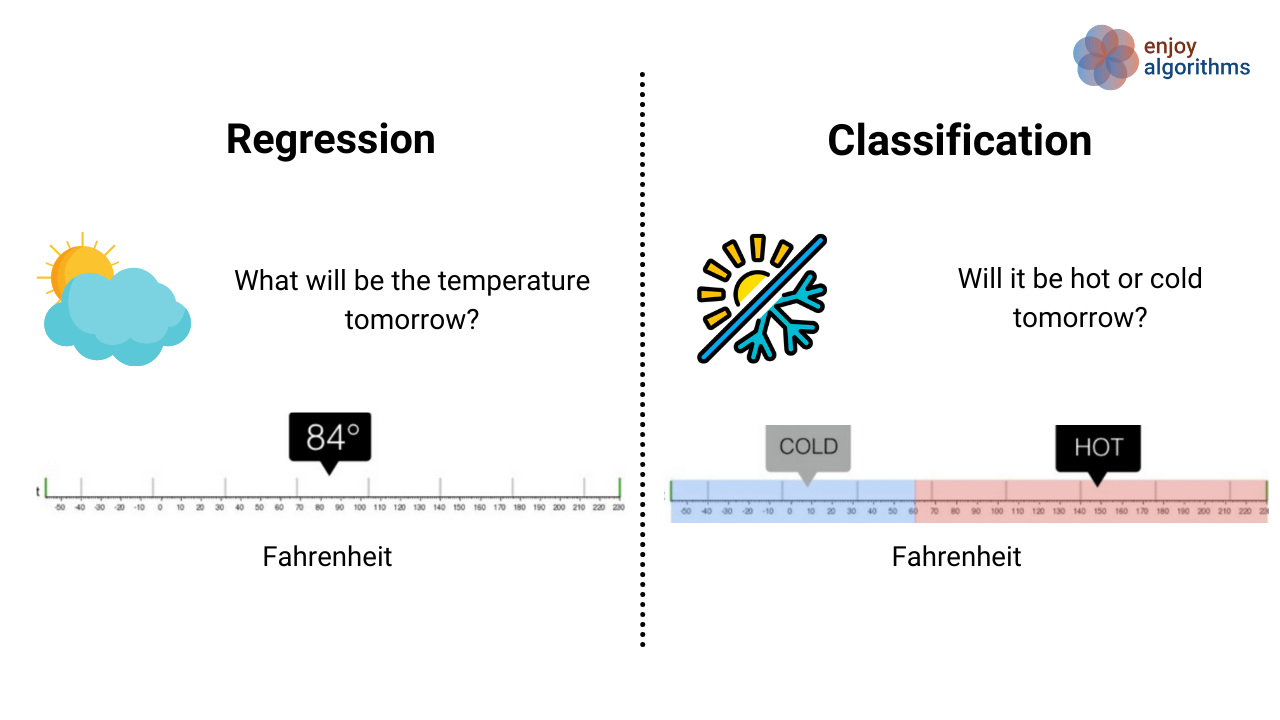
\includegraphics[scale=0.25]{images/regression vs classification.png} 
\end{center}
\end{frame}

\subsection[Algorithmes Courants]{Algorithmes Courants}
\begin{frame}
\frametitle{Algorithmes Courants}
\setbeamercolor{block title}{use=structure,fg=white,bg=blue!75!black}
\setbeamercolor{block body}{use=structure,fg=black,bg=white!20!white}
\begin{block}{Algorithmes Courants}
\begin{itemize}
	\item Régression Linéaire (régression)
	\item Régression Logistique (classification)
	\item Arbres de Décision
	\item k-Nearest Neighbors (k-NN)
	\item Support Vector Machine (SVM)
\end{itemize}
\end{block}
\end{frame}

\subsection[Étapes de Fonctionnement]{Étapes de Fonctionnement}
\begin{frame}
	\frametitle{Étapes de Fonctionnement}
	\setbeamercolor{block title}{use=structure,fg=white,bg=blue!75!black}
	\setbeamercolor{block body}{use=structure,fg=black,bg=white!20!white}
	\begin{block}{Étapes de Fonctionnement}
		\begin{enumerate}
			\item Collecte de données étiquetées
			\pause
			\item Séparation en données d'entraînement et de test
			\pause
			\item Entraîner le modèle en utilisant les données d'entraînement
			\pause
			\item Évaluer la performance du modèle sur les données de test
			\pause
			\item Deployer le modèle en production
		\end{enumerate}
	\end{block}
	\begin{block}{Évaluation du Modèle}
		\begin{itemize}
			\item Précision – Nombre de bonnes prédictions
			\item Recall et F1 Score – Pour la classification
			\item Erreur Quadratique Moyenne (MSE) – Pour la régression
		\end{itemize}
	\end{block}
\end{frame}

\end{document}
